\documentclass{aip-cp}

\usepackage[numbers]{natbib}
\usepackage{rotating}
\usepackage{graphicx}
\usepackage{dirtytalk}

\usepackage{url}

\let\iint\relax
\let\iiint\relax
\let\iiiint\relax
\let\idotsint\relax
\usepackage{amsmath}

\newcommand*\Laplace{\mathop{}\!\mathbin\bigtriangleup}
\newcommand{\figref}[1]{\figurename~\ref{#1}}
\newcommand{\tabref}[1]{\tablename~\ref{#1}}
\newcommand{\norm}[1]{\left\lVert#1\right\rVert}

\DeclareMathOperator*{\argmin}{arg\,min}
\DeclareMathOperator*{\argmax}{arg\,max}

\usepackage{xcolor}
\usepackage{colortbl}
\definecolor{LightCyan}{rgb}{0.82,1,1}
\definecolor{Cyan}{rgb}{0.60,1,1}

\begin{document}

% Title portion
\title{Image features classification using Bayesian model}

\author[aff1,aff2]{Vojt\v{e}ch Dor\v{n}\'{a}k}
\author[aff1]{Luk\'{a}\v{s} Posp\'{i}\v{s}il\corref{cor1}}
\author[aff2]{Marek Pecha}
\author[aff1]{Martin \v{C}erm\'{a}k}

\affil[aff1]{Department of Mathematics, Faculty of Civil Engineering, VSB-TU Ostrava, Czech Republic}
\affil[aff2]{Department of Applied Mathematics, FEECS, VSB-TU Ostrava, Czech Republic}
\corresp[cor1]{Corresponding author: lukas.pospisil@vsb.cz}

\maketitle

\begin{abstract}
    This paper presents the first results of the Bayesian model in the problem of image classification using feature extraction. The proposed approach is similar to the well-known Markov processes and is based on conditional probabilities determined from the given data using the regression process with Kullback-Leibler divergence. In the contribution, we shortly review the complete process consisting of the Scale Invariant Feature Transform technique for the detection of key features, Bag of Visual Words, and classification. We compare the new methodology with the standard approach based on Support Vector Machine on a non-trivial benchmark containing real photographs of cats and dogs.
\end{abstract}

\maketitle

\section{Introduction}
In this paper, we introduce the Bayesian model and the Support Vector Machine classification techniques. We experiment with these techniques on classifying photographs of cats and dogs from the Oxford-IIIT Pet Dataset \cite{parkhi12a}, transformed into a space of significant features using the Scale Invariant Feature Transform technique \cite{Lowe2004}.

It has been shown in \cite{dornak2020}, that classifying the transformed data using the Support Vector Machine is a viable option. In \cite{dornak2021}, these classification techniques have been explored on multiple different datasets. In this paper, we compare the results of the two classification techniques mentioned above.

\section{Scale Invariant Feature Transform}
Scale Invariant Feature Transform (SIFT) is a commonly used local feature extractor, firstly proposed by David Lowe in 2004 \cite{Lowe2004}. It describes an area around a few selected key points by the means of a vector called a descriptor. These descriptors are invariant to scale, rotation, illumination and affine transformations.

Let the scale-space representation of an image $L(x,y,\sigma)$ be the convolution of the input image with the Gaussian kernel. The scale-invariant key points are selected as extrema of the scale normalized Laplacian of Gaussian (LoG):
\begin{equation}
    \Laplace_{norm} L(x, y, \sigma) = \sigma \left(\frac{\partial^2 L(x,y,\sigma)}{\partial x^2} + \frac{\partial^2 L(x,y,\sigma)}{\partial y^2}\right).
\end{equation}

Since the determination and the evaluation of LoG is time-consuming, it is approximated by the Difference of Gaussian (DoG). The DoG is computed by subtracting two adjacent scale-space representations of the image, which is performed across different scales, where the scales are constructed by progressively convolving the original image with the Gaussian kernel.

Each candidate pixel is compared with the 8 surrounding pixels as well as with the 9 pixels in the scale above and the 9 pixels in the scale below. If the candidate pixel intensity is lower or higher than the 26 surrounding pixels, it is selected as a key point. To detect the sub-pixel location of extrema, the DoG is interpolated using a quadratic Taylor expansion at each candidate. The key point is discarded, if the offset from the key point is greater than $0.5$ in any dimension, as this indicates that the extremum is close to a better key point. key points located along edges are also considered poorly located and therefore are discarded.

The key point descriptors for the object must be almost identical across different scales, rotations, illuminations and other transformations. To ensure descriptor invariance to rotation, the key point orientation needs to be determined. It is selected as a dominant gradient magnitude, from an orientation histogram.

The descriptor is constructed from a window of a size $16 \times 16$ pixels around the key point. This window is rotated according to the previously selected orientation of the key point. The window is divided into 16 ($4 \times 4$) sub-windows. In each sub-window, an $8$ bin histogram weighted by the gradient magnitudes is constructed. These histograms form a descriptor vector.

The SIFT extractor provides us with a various number of descriptors for each image. Since we require each image to be represented by a single vector, we apply the Bag of Words technique (BoW). The BoW represents each sample in a dataset as a multi-set of its words. In our case, the words are a categorization of descriptors from all images. The categorization is done using $k$-means clustering.

\section{Support Vector Machines}
The Support Vector Machine is a supervised learning model designed for binary data classification \cite{boser1992}. It is well known and commonly used for classification in various fields. In the case of image classification, promising results have been proposed in \cite{dornak2020}.

Let $T := \{(\boldsymbol{x_1}, y_1),(\boldsymbol{x_2}, y_2),...,(\boldsymbol{x_n}, y_n)\}$,
be the training dataset, where $n$ is the number of the samples, $\boldsymbol{x_i} \in \mathbb{R}^m$, $i \in \{1,2,\dots,n\}$,
are samples and $y_i \in \{-1, 1\}$ are corresponding sample labels. The classification model is represented in the form of the hyperplane $H: \boldsymbol{\omega}^\top\boldsymbol{x}-\widetilde{b}=0$, where $\boldsymbol{\omega} \in \mathbb{R}^{m}$ is the normalized normal vector of the hyperplane $H$, and $\widetilde{b} = \frac{b}{\norm{\boldsymbol{\omega}}} \in \mathbb{R}$ is the bias from the origin.

By augmenting the vector $\boldsymbol{\omega}$ and each sample $\boldsymbol{x_i}$ with an additional auxiliary dimension, so that $\boldsymbol{\widehat{\omega}} \leftarrow \begin{bmatrix}\boldsymbol{\omega} & B \end{bmatrix}^\top$, $\boldsymbol{\widehat{x}_i} \leftarrow \begin{bmatrix}\boldsymbol{x}_i & \beta \end{bmatrix}^\top$, where $B \in \mathbb{R}$, and $\beta \in \mathbb{R}^+$ is a user defined variable, the relaxed bias $\widetilde{b}$ is included in the problem. Such approach is well known as the no-bias classification \cite{Aeta2018}.

The hyperplane $H: \boldsymbol{\widehat{\omega}}^\top\boldsymbol{\widehat{x}}=0$ can be determined using a constrained optimization problem in the primal formulation:
\begin{equation}
    \argmin_{\boldsymbol{\widehat{\omega}},\xi_i} \frac{1}{2}\|\boldsymbol{\widehat{\omega}}\|^2 + \frac{C}{p}\sum_{i = 1}^n\xi_i^p ~~\text{ s.t. } ~~
    \begin{cases}
        y_i(\boldsymbol{\widehat{\omega}}^\top\boldsymbol{\widehat{x_i}})\geq1 - \xi_i,\\
        \xi_i \geq 0 \text{ if } p=1, i=1, ...,n,
    \end{cases}
    \label{eq:svm:primal}
\end{equation}
where $\xi_i = \max(0, 1-y_i(\boldsymbol{\widehat{\omega}}^\top\boldsymbol{\widehat{x_i}}))$ is the hinge loss function, $C \in \mathbb{R}^+$ is a penalty, that penalizes misclassification error. The appropriate penalty $C$ can be determined using the grid-search technique combined with cross-validation method.

Exploiting the Lagrange duality and evaluating the Karush-Kuhn-Tucker conditions for \eqref{eq:svm:primal},
we obtain the $l1$-loss $l2$-regularized SVM formulation:
\begin{equation}
    \argmin_{\boldsymbol{\lambda}} \ \frac{1}{2} \boldsymbol{\lambda}^\top \boldsymbol{H}  \boldsymbol{\lambda} -  \boldsymbol{\lambda}^\top \boldsymbol{e} ~~\text{ s.t. }~~ \boldsymbol{o} \leq  \boldsymbol{\lambda} \leq C\boldsymbol{e},
    \label{eq:svm:dualL1}
\end{equation}
for $p=1$. For $p=2$, we get the $l2$-loss $l2$-regularized SVM formulation:
\begin{equation}
    \argmin_{\boldsymbol{\lambda}} \ \frac{1}{2} \boldsymbol{\lambda}^\top \left(\boldsymbol{H} + C^{-1} \boldsymbol{I} \right) \boldsymbol{\lambda} -  \boldsymbol{\lambda}^\top \boldsymbol{e} ~~\text{ s.t. }~~    \boldsymbol{o} \leq  \boldsymbol{\lambda}.
    \label{eq:svm:dualL2}
\end{equation}

In the proposed optimization problems, $\boldsymbol{H} = \boldsymbol{Y}^\top \boldsymbol{G} \boldsymbol{Y}$, $\boldsymbol{G} = \boldsymbol{X}^\top\boldsymbol{X}$ denotes the Gramian matrix, $\boldsymbol{X}= \begin{bmatrix} \boldsymbol{\widehat{x}}_1 & \dots & \boldsymbol{\widehat{x}}_n \end{bmatrix}$, $\boldsymbol{Y} = diag(\boldsymbol{y})$, $\boldsymbol{y} = \left[y_1, \ y_2, \  \dots, y_n\right]^\top$, $\boldsymbol{e} = \left[1, 1, \dots, 1\right]^\top \in \mathbb{R}^n$, $\boldsymbol{o} = \left[0, \ 0,  \ \dots, \ 0\right]^\top \in \mathbb{R}^n$.

In the $l2$-loss $l2$-regularized SVM formulation, the Hessian matrix $\boldsymbol{H}$ regularized by the matrix $C^{-1}\boldsymbol{I}$ is symmetric positive definite. In this case, the objective function is strictly convex and the problem \eqref{eq:svm:dualL2} has unique solution \cite{DosBOOK-2009}.

\section{Bayesian Model}

The method is based on law of total probability for two categorical processes. 
Let $x_t \in X \coloneqq \lbrace \mathsf{x}_1, \dots \mathsf{x}_{K_x} \rbrace, t = 1,\dots,T$ be the input variables and let $y_t \in \mathsf{Y} := \lbrace \mathsf{y}_1, \dots, \mathsf{y}_{K_Y} \rbrace$ be output labels.
Let $\Pi_{xt}^{K_y}$ be a stochastic vector of relative frequences of word categories $X$ in image $t$ and $\Pi_{yt} \in \mathbb{R}^{K_y}$ be a vector of probabilities of image classification. Then using on the law of total probability, there exists a left stochastic matrix of conditional probabilities $\Lambda \in \mathbb{R}^{K_y,K_x}$ with components
\begin{equation}
    \Lambda_{ij} = P(y_t = \mathsf{y}_i | x_t = \mathsf{x}_j), i = 1, \dots, K_y, j = 1, \dots, K_x.
\end{equation}

%This classifier is suitable for classifying data represented by a stochastic vector. The BoW data can be easily transformed into such vector. Instead of each component of the BoW vector representing the number of key points in the respective category, the component in our new vector represents the probability of key points belonging to the respective category.
%Let us denote the stochastic data vector $\Pi_{xt} \in \mathbb{R}^{K_x}, t=1,\dots,T$, where $T$ is the number of samples, $K_x$ is the size of BoW. Let the vector $\Pi_{yt}\in \mathbb{R}^{K_y}$ be a vector of probabilities, with which $\Pi_{xt}$ belongs to each category, and $K_y$ the number of categories.
%Given a stochastic data vector $\Pi_x$, we can describe the transformation $\mathbb{R}^{K_x} \rightarrow \mathbb{R}^{K_y}$ using a matrix $\Lambda \in \mathbb{R}^{K_y, K_x}$:
%where $\Pi_x^n$ is the $n$-th element of $\Pi_x$, similar to $\Pi_y^n$, and the matrix $\Lambda$ is a left stochastic matrix.

The determination of the optimal $\Lambda^{*}$ can be written as regression problem
\begin{equation}
    \Lambda^* = \argmin_{\Lambda \in \Omega_{\Lambda}} \sum_{t=1}^{T} \text{dist}(\Pi_{yt}, \Lambda\Pi_{xt}),
    \label{eq:Bayes:opt_problem}
\end{equation}
where $\Omega_{\Lambda}$ is a feasible set of left stochastic matrices. In our approach, the dist($\Pi_{yt}, \Lambda\Pi_{xt}$) is chosen as Kullback-Leiber divergence \cite{Kullback1951}:
\begin{equation}
    \text{dist}(\Pi_{yt}, \Lambda\Pi_{xt}) = - \sum_{i=1}^{K_y} \Pi_{yt}^i \ln\frac{[\Lambda\Pi_{xt}]_i}{[\Pi_{yt}]_i} = - \sum_{i=1}^{K_y} [\Pi_{yt}]_i (\ln [\Lambda\Pi_{xt}]_i - \ln [\Pi_{yt}]_i)
    \propto - \sum_{i=1}^{K_y} [\Pi_{yt}]_i \ln [\Lambda\Pi_{xt}]_i.
\end{equation}
Since the objective function of \eqref{eq:Bayes:opt_problem} is convex, we can use Jensen's inequality to obtain
\begin{equation}
\label{eq:jensen}
    - \sum_{i=1}^{K_y} [\Pi_{yt}]_i \ln [\Lambda\Pi_{xt}]_i \leq - \sum_{i=1}^{K_y} [\Pi_{yt}]_i ( \sum_{j=1}^{K_x} [\Pi_{xt}]_j \ln (\Lambda_{ij}) ) = - \sum_{i=1}^{K_y} \sum_{j=1}^{K_x} [\Pi_{yt}]_i [\Pi_{xt}]_j \ln \Lambda_{ij}.
\end{equation}
%From this estimation, we get an approximated optimization problem
%\begin{equation}
%    \Lambda^* = \argmin_{\Lambda \in \Omega_{\Lambda}} - \sum_{t=1}^{T} \sum_{i=1}^{K_y} \sum_{j=1}^{K_x} [\Pi_{yt}]_i [\Pi_{xt}]_j \ln \Lambda_{ij},
%\end{equation}
%where $\Omega_{\Lambda} = \{ \Lambda \in [0, 1]^{K_y,K_x}, \forall j \in \{ 1, 2, \dots, K_x \} : \sum_{i=1}^{K_y} \Lambda_{ij} = 1 \}$
%is a feasible set of left stochastic matrices. 
The problem \eqref{eq:Bayes:opt_problem} with objective function \eqref{eq:jensen} has analytical solution, which can be derived using Lagrange multipliers
\begin{equation}
\label{eq:Lambda_est}
    \Lambda_{\hat{i}\hat{j}}^{*} = \frac{\sum_{t=1}^{T} [\Pi_{yt}]_{\hat{i}} [\Pi_{xt}]_{\hat{j}}}{\sum_{i=1}^{K_y} \sum_{t=1}^{T} [\Pi_{yt}]_{i} [\Pi_{xt}]_{\hat{j}},}.
\end{equation}
Please notice the similarity of obtained formula with the estimation of the Markov chain transitional matrix estimated by Matimum Likelihood Principle \cite{NorBOOK-1998}.
In this paper, we compare solution \eqref{eq:Lambda_est} with numerical solution of original problem \eqref{eq:Bayes:opt_problem} without using the Jensen's inequality. Since the feasible set $\Omega_{\Lambda}$ is a closed convex set and we can easily derive the derivatives of objective function, the problem can be solved numerically using the Spectral Projected Gradient method \cite{birgin2000}. We compare both approaches in our experiments.

\section{Benchmark Results}
To test our extraction-classification pipeline, we use the Oxford-IIIT Pet Dataset \cite{parkhi12a}. The dataset contains over $7,000$ photographs of different cat and dog breeds. The dataset provides a trimap for each photograph, allowing us to cut out the animal from the background. This allows us to concentrate only on classifying the data relevant to the animal. We assign $90\%$ of the data to the training subset and $10\%$ to the testing subset.

We run the presented experiments on the Salomon supercomputer \cite{Salomon-WWW-17} at IT4Innovations. As the underlying SVM solver, we use PermonSVM \cite{permonSVM}. The Bayesian Model using the Jensen inequality is implemented in Python, while the Bayesian Model solved using the Spectral Projected Gradient method is trained using an Octave code.

\begin{figure}[!ht]
    \centering
    \begin{minipage}{.5\textwidth}
        \centering
        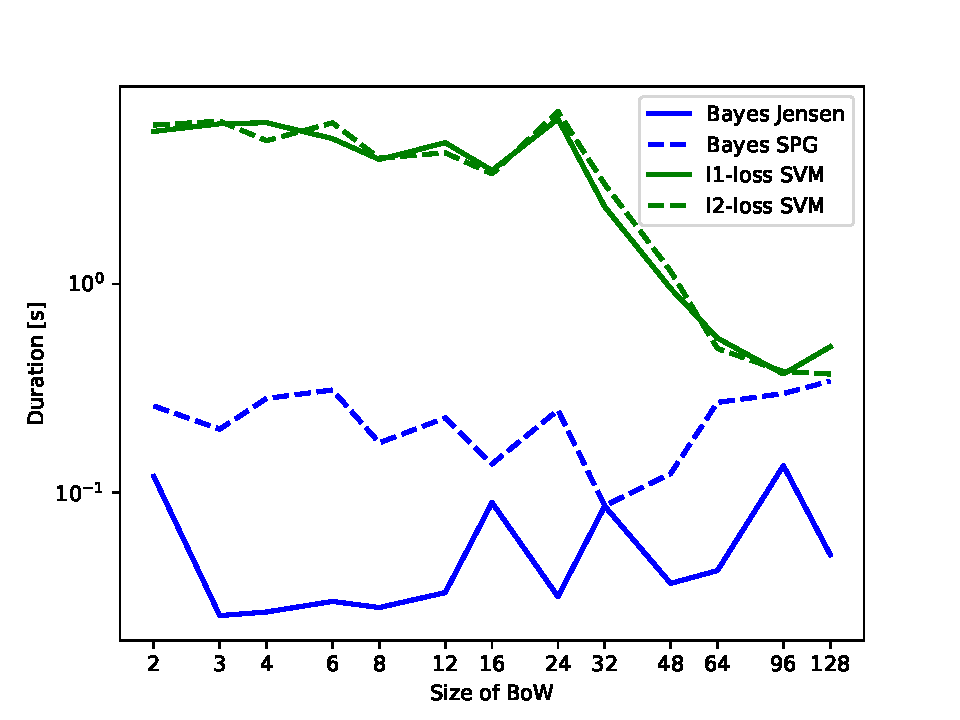
\includegraphics[width=\textwidth]{Figures/times.pdf}
    \end{minipage}%
    \begin{minipage}{.5\textwidth}
        \centering
        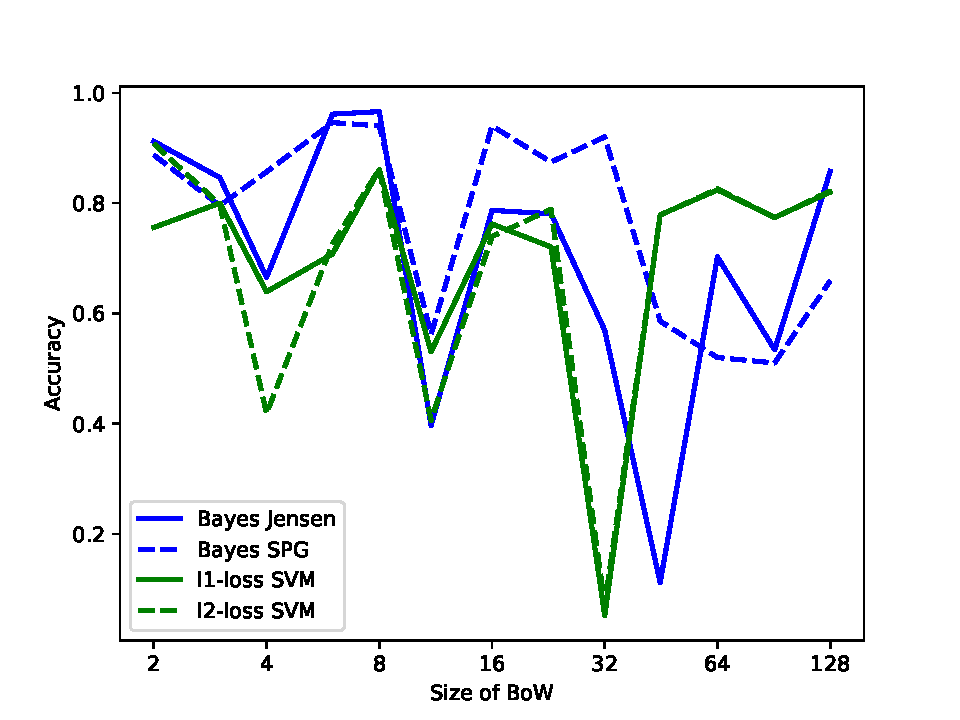
\includegraphics[width=\textwidth]{Figures/score.pdf}
    \end{minipage}
    \caption{The results of image classification benchmark: the computational time (left, lower is better) and the classification accuracy of proposed methods (right, higher is better).}
    \label{fig:results:graph}
\end{figure}

From the graphs in \figref{fig:results:graph}, we can observe that for the lower BoW sizes both versions of the Bayes classifier perform better in regards to accuracy and the duration of training. However, with the larger BoW sizes, both the $l1$-loss and the $l2$-loss regularized SVM performs similarly to the Bayes classifier.

\section{Conclusion}
In our contribution, we presented the Bayesian model in image classification and demonstrated the efficiency of this novel approach on the standard non-trivial benchmark. Our first results indicate better performance than commonly used SVM. Additionally, our method can be easily extended to the classification of images into more classes, whereas the SVM approach can be directly used only for binary classification. However, this feature as well as the comparison to other commonly used techniques (such as Neural Networks) would provide a better understanding of the efficiency of this promising method. This will be the aim of our further research.

\section{Acknowledgement}
This contribution has been developed as a part of the research project GACR 21-14886S ``Influence of Material Properties of High Strength Steels on Durability of Engineering Structures and Bridges'' supported by the Czech Grant Agency and the financial support provided to VSB-Technical University of Ostrava by the Czech Ministry of Education, Youth and Sports from the budget for conceptual development of science, research and innovations for the 2021 year.

\bibliographystyle{aipnum-cp}
\bibliography{DorCer_icnaam2021}

\end{document}
